\documentclass[10pt,conference]{IEEEtran}

% ============================================================
% Packages
% ============================================================
\usepackage[T1]{fontenc}
\usepackage[utf8]{inputenc}
\usepackage{times}
\usepackage{microtype}
\usepackage{graphicx}
\usepackage{booktabs}
\usepackage{array}
\usepackage{tabularx}
\usepackage{enumitem}
\usepackage{xcolor}
\usepackage{hyperref}
\usepackage{listings}
\usepackage{amsmath}
\usepackage{amssymb}
\usepackage{multirow}
\usepackage{caption}

\hypersetup{
    colorlinks=true,
    linkcolor=blue,
    citecolor=blue,
    urlcolor=blue
}

\setlist[itemize]{leftmargin=*, itemsep=2pt, topsep=2pt}
\setlist[enumerate]{leftmargin=*, itemsep=2pt, topsep=2pt}

\lstset{
    basicstyle=\footnotesize\ttfamily,
    breaklines=true,
    frame=single,
    columns=fullflexible,
    keepspaces=true,
    showstringspaces=false
}

% ============================================================
% Title
% ============================================================
\title{
Shakespeare-Aware Language System Using\\Retrieval-Augmented Generation with a Small Language Model
}

\author{
\IEEEauthorblockN{
Group Number: \emph{[Insert Group Number]}
}
\IEEEauthorblockA{
CSCI433/933 Machine Learning Algorithms and Applications\\
Student Names and Student Numbers: \emph{[Insert Details]}\\
}
}

\begin{document}
\maketitle

% ============================================================
% Page Limit Notice
% ============================================================
\begin{center}
\fbox{
\begin{minipage}{0.94\linewidth}
\textbf{Main Report Page Limit:} The main report must not exceed \textbf{10 pages}, in the style of IEEE conference submissions.
The 10-page (absolute) limit applies from the abstract through the conclusion.
References, appendices, full evaluation tables, extended prompts, and the GenAI usage log are excluded from the 10-page limit.
\end{minipage}
}
\end{center}

% ============================================================
% Abstract
% ============================================================
\begin{abstract}
In this report, we describe a Shakespeare-aware question answering system that uses Retrieval-Augmented Generation (RAG) with a Small Language Model (SLM). The system helps users who do not have Shakespeare background to ask questions about three plays---\textit{Hamlet}, \textit{Macbeth}, and \textit{Romeo and Juliet}---and get easy-to-understand answers based on the actual text. We use TinyLlama-1.1B-Chat for text generation and sentence-transformers/all-MiniLM-L6-v2 for embeddings. We chunk the text at scene level and add summary and keywords to each chunk to help the retrieval. We also cache the embeddings on disk so the system starts faster after the first run. We test the system with 15 questions covering five types: contextual QA, concept explanation, evidence retrieval, stylised generation, and robustness. The results show that RAG clearly improves the answer quality compared to a prompt-only baseline. However, both systems still have problems like hallucination and not following instructions well, which is expected for a small 1.1B model.
\end{abstract}

% ============================================================
\section{Introduction and Problem Formulation}
\label{sec:introduction}

In this project, we try to adapt a pretrained Small Language Model (SLM) so that it can answer questions about Shakespeare's plays. This is basically a domain adaptation problem, because Shakespearean English is very different from modern English in terms of vocabulary, grammar, and expressions. Most pretrained models are trained on modern text, so they may not know the details of Shakespeare's plays very well.

\textbf{Problem statement.} Our goal is to build a system that can help someone who has never read Shakespeare before. The user can ask questions about three plays---\textit{Hamlet}, \textit{Macbeth}, and \textit{Romeo and Juliet}---and get clear, easy-to-understand answers that are based on the actual play text. The system needs to support four types of interaction: concept explanation, contextual QA, evidence retrieval, and stylised generation.

\textbf{Why Shakespeare is hard for a model.} Shakespeare uses old words like ``thee'', ``hath'', ``wherefore'', and the sentence structure is very different from modern English. A pretrained model might have learned some general knowledge about Shakespeare, but it can easily get the details wrong, like character relationships or specific plot events. This is why we use Retrieval-Augmented Generation (RAG)---we give the model the actual text from the plays as context, instead of just relying on what it already knows.

\textbf{Target user.} We design the system for beginners who do not have any background in Shakespeare. The answers should be clear and avoid using difficult literary terms.

\textbf{Design constraints.} Based on the assignment requirements, our system must:
\begin{itemize}
    \item use a pretrained SLM, not train from scratch;
    \item have a RAG pipeline;
    \item be able to run on a normal laptop;
    \item make it clear when the output is creative writing vs. factual answer.
\end{itemize}

Because of these constraints, we chose a small 1.1B-parameter model, simple cosine similarity for retrieval, and scene-level chunking with extra metadata.

% ============================================================
\section{Dataset and Preprocessing}
\label{sec:dataset}

\subsection{Dataset Description}

The dataset has three JSON files, one for each play. The instructor provided these files, and they were originally from Project Gutenberg. The data is already structured in a hierarchy like this:

\begin{center}
\texttt{Play $\rightarrow$ Act $\rightarrow$ Scene $\rightarrow$ Speaker $\rightarrow$ Utterance}
\end{center}

Table~\ref{tab:dataset-stats} shows the basic statistics of the dataset.

\begin{table}[h]
\centering
\caption{Dataset statistics for the three compulsory plays.}
\label{tab:dataset-stats}
\begin{tabular}{lccc}
\toprule
Play & Scenes & Utterances & Avg. Words/Scene \\
\midrule
Hamlet & 20 & 1,657 & $\sim$1,200 \\
Macbeth & 28 & 830 & $\sim$550 \\
Romeo and Juliet & 25 & 1,126 & $\sim$750 \\
\midrule
\textbf{Total} & \textbf{73} & \textbf{3,613} & --- \\
\bottomrule
\end{tabular}
\end{table}

\subsection{Dataset Schema}

Each scene record keeps the following metadata:

\begin{lstlisting}[language={}]
{
  "scene_id": "macbeth_1_3",
  "play": "Macbeth",
  "act": 1,
  "scene": 3,
  "location": "A heath. Thunder",
  "scene_summary": "The witches greet Macbeth
    with prophecies...",
  "keywords": ["prophecy", "ambition"],
  "utterances": [ ... ],
  "text": "...full scene text..."
}
\end{lstlisting}

The \texttt{scene\_summary} and \texttt{keywords} fields are already in the dataset. They are written in modern English and help explain what each scene is about. We use them as supplementary information to help connect the user's modern English query with the old Shakespearean text. In our system, we put these annotations at the top of each chunk as headers, and the original Shakespeare text comes after them. This way, the primary text and the supplementary material are clearly separated.

\subsection{Chunking Strategy}

We use a \textbf{scene-level chunking strategy with summary and keyword enrichment}. For each scene, we make one retrieval chunk by putting the summary, keywords, and location at the top, followed by the original scene text:

\begin{lstlisting}[language={}]
Summary: <scene_summary>
Keywords: <keyword1>, <keyword2>
Location: <location>
<original scene text>
\end{lstlisting}

\textbf{Why scene-level.} We chose scene-level because it keeps the whole conversation between characters together, so the context is not broken. If we used utterance-level, each chunk would be just one line from one speaker, and you would lose the relationship between characters in that scene. Adding the summary at the top also helps, because the summary is in modern English, which makes it easier for the embedding model to match with the user's question.

\textbf{Handling long scenes.} Some scenes have more than 4,000 characters, which is too long for the embedding model to handle well (MiniLM-L6-v2 can only process about 256 tokens). For these long scenes, we split them into smaller sub-chunks with 400 characters of overlap at sentence boundaries, so we do not lose context between the parts. After splitting, we get about 80 chunks from the original 73 scenes.

\textbf{Trade-offs.} Scene-level chunks are bigger than utterance-level chunks, so if a question is about one specific line, the retrieval might be less precise. But in practice, the summary at the top of each chunk works like a semantic anchor, and in our tests, the system usually retrieves the right scene for most questions.

% ============================================================
\section{Methodology}
\label{sec:methodology}

\subsection{Baseline System}

Our baseline is a \textbf{prompt-only system}. It just sends the user's question to the language model directly, without giving it any context from the plays. The prompt looks like this:

\begin{lstlisting}[language={}]
You are a helpful assistant that answers
questions about Shakespeare's plays.
Answer in a beginner-friendly way. If you
are unsure, say so.

Question: <user query>

Answer:
\end{lstlisting}

We use the \textit{same model} (TinyLlama-1.1B-Chat) and \textit{same generation parameters} (temperature = 0.7, top\_p = 0.9, max\_new\_tokens = 512) for both the baseline and the RAG system. The only difference is that the baseline does not get any retrieved context. This way, the comparison is fair---if the RAG system gives better answers, we know it is because of the retrieval part.

\textbf{Why this baseline is fair.} The prompt-only approach is the simplest possible system. It only uses what the model learned during pretraining. Since TinyLlama was trained on a lot of text data, it probably has some knowledge about Shakespeare already, so the baseline is not completely useless. It gives us a reasonable lower bound to compare with.

\subsection{RAG-Based System}

The RAG system adds retrieved evidence from the Shakespeare plays to help the language model give better answers. The pipeline works like this:

\begin{enumerate}
    \item \textbf{Query embedding}: We use MiniLM-L6-v2 to turn the user's question into a vector.
    \item \textbf{Retrieval}: We calculate cosine similarity between the query vector and all chunk vectors, then return the top-$k$ ($k=3$) most similar chunks.
    \item \textbf{Prompt construction}: We put together the system prompt, the retrieved passages (with metadata like play name, act, scene), and the user's question into one prompt.
    \item \textbf{Generation}: TinyLlama reads the whole prompt and generates an answer.
    \item \textbf{Evidence display}: We show the retrieved passages next to the answer, with their source information and similarity scores.
\end{enumerate}

The RAG prompt uses a system instruction that we store in \texttt{prompts/system\_prompt.txt}:

\begin{lstlisting}[language={}]
You are a Shakespeare-aware assistant.
Use the retrieved context to answer the
user's question.
Your answer must be beginner-friendly.
If the retrieved context is insufficient,
say so clearly.
Do not invent unsupported details.
If asked to produce a Shakespearean-style
response, keep it under 150 words and make
clear that it is creative output, not
textual evidence.
\end{lstlisting}

Each retrieved passage is shown with its source information:

\begin{lstlisting}[language={}]
[Source 1: Macbeth, Act 2, Scene 2
 | relevance=0.740]
Summary: Macbeth murders Duncan...
<scene text excerpt>
\end{lstlisting}

\textbf{Stylised generation.} If the user asks for a Shakespearean-style response, the system detects this automatically by checking for keywords like ``shakespearean'', ``style of'', or ``generate''. When this happens, we use a different prompt that tells the model to write a short creative response ($\leq$150 words) in old English style. The output is always labelled with a note at the top: \texttt{[NOTE: The following is creative Shakespearean-style output, not factual evidence.]} so the user knows it is not factual.

\subsection{Model Choice and Justification}

\textbf{Generation model: TinyLlama-1.1B-Chat-v1.0.} This is a 1.1 billion parameter model that has been fine-tuned for chat. We chose it because:
\begin{itemize}
    \item \textbf{Small size}: It is only about 2~GB (FP16), so it can run on a normal laptop with 8~GB RAM.
    \item \textbf{Chat ability}: Because it is fine-tuned for chat, it can follow instructions in the prompt, which is important for our system.
    \item \textbf{Easy to use}: It is free on HuggingFace and does not need any API key.
\end{itemize}

We load the model only once using a singleton pattern in \texttt{src/model.py}, and both the baseline and RAG systems share the same model. This saves memory and makes sure the generation is consistent.

\textbf{Embedding model: sentence-transformers/all-MiniLM-L6-v2.} This is a small embedding model (22M parameters) that converts text into 384-dimensional vectors. It is a popular choice for semantic search and runs fast on CPU---it takes about 10 seconds to embed all 73 chunks. We did not use bigger embedding models like BGE because for our small dataset, the improvement would be very small but the cost would be higher.

\textbf{Retrieval method: cosine similarity with scikit-learn.} We use scikit-learn's \texttt{cosine\_similarity} to compare the query vector with all chunk vectors. Since we only have about 80 chunks, this is very fast and we do not need heavy tools like FAISS or Chroma. Keeping it simple also makes the code easier to understand and debug.

% ============================================================
\section{System Design and Implementation}
\label{sec:system}

\subsection{System Pipeline}

Figure~\ref{fig:pipeline} shows how the whole RAG pipeline works.

\begin{figure}[h]
\centering
\begin{lstlisting}[language={},frame=none]
User Query
    |
    v
[Embed Query] --> [Cosine Similarity]
  (MiniLM)        (against 73+ chunks)
                        |
                   top-k chunks
                        |
                        v
              [Build RAG Prompt]
              (system prompt +
               retrieved text +
               user question)
                        |
                        v
              [TinyLlama Generate]
                        |
                        v
              [Display Answer +
               Retrieved Evidence]
\end{lstlisting}
\caption{End-to-end RAG pipeline.}
\label{fig:pipeline}
\end{figure}

\subsection{Implementation Details}

\textbf{Language and libraries.} We use Python 3.9+ with the following main libraries: \texttt{torch}, \texttt{transformers}, \texttt{sentence-transformers}, \texttt{scikit-learn}, \texttt{numpy}, \texttt{pandas}, and \texttt{tqdm}.

\textbf{Repository structure.} Our project folder is organised like this:

\begin{lstlisting}[language={},frame=none]
assignment2_starter_code/
  data/processed/      (3 play JSON files)
  data/cache/          (embedding cache)
  prompts/             (system_prompt.txt)
  results/             (questions, CSV output)
  src/                 (all Python modules)
  report/              (this report)
  requirements.txt
  README.md
\end{lstlisting}

\textbf{How to run the system:}
\begin{enumerate}
    \item \texttt{pip install -r requirements.txt}
    \item \texttt{python src/build\_index.py} --- test retrieval pipeline (no LLM)
    \item \texttt{python src/rag\_chatbot.py} --- interactive RAG chatbot
    \item \texttt{python src/evaluate.py} --- run full evaluation
\end{enumerate}

\textbf{Embedding caching.} The first time you run the system, it computes embeddings for all chunks and saves them to \texttt{data/cache/embeddings\_<hash>.pkl}. The hash is based on the model name and an MD5 of all the chunk texts. Next time you run it, the embeddings load from the cache file instantly. If you change the chunking or the embedding model, the hash will be different, so the cache will be recomputed automatically.

\textbf{Environment issues.} We found that on some Windows machines, importing \texttt{transformers} can crash because of a broken \texttt{h5py} DLL. To fix this, we set some environment variables in \texttt{config.py} to prevent TensorFlow from loading, and we also inject a fake \texttt{h5py} module. This way, the system works without needing TensorFlow installed.

\textbf{Known limitations.}
\begin{itemize}
    \item TinyLlama can only handle 2,048 tokens at a time, so we have to cut long retrieved passages.
    \item We only have a command-line interface, no web UI.
    \item The retrieval is just brute-force cosine similarity. This is fine for our 80 chunks, but it would be slow if the dataset was much bigger.
\end{itemize}

% ============================================================
\section{Evaluation Design}
\label{sec:evaluation-design}

\subsection{Evaluation Questions}

We test our system with \textbf{15 questions} from two sources and five different types. Table~\ref{tab:question-dist} shows the breakdown.

\begin{table}[h]
\centering
\caption{Evaluation question distribution.}
\label{tab:question-dist}
\begin{tabular}{llcc}
\toprule
Source & Type & Count & Plays \\
\midrule
Instructor & contextual\_qa & 6 & All 3 \\
\midrule
Group & concept\_explanation & 3 & All 3 \\
Group & evidence\_retrieval & 2 & Mac, Ham \\
Group & contextual\_qa & 1 & R\&J \\
Group & stylised\_generation & 2 & Mac, Ham \\
Group & robustness & 1 & N/A \\
\midrule
\textbf{Total} & & \textbf{15} & \\
\bottomrule
\end{tabular}
\end{table}

The 6 \textbf{instructor questions} (Q1--Q6) are all contextual QA questions covering all three plays. We also designed 9 \textbf{group questions} to test more things: concept explanation (G1--G3), evidence retrieval (G4--G5), one more contextual QA (G6), stylised generation (G7--G8), and one robustness test (G9). For G9, we deliberately asked an out-of-domain question (``Who is Mingzhao Zhu?'') to see if the system can handle questions that have nothing to do with Shakespeare.

\subsection{Scoring Criteria}

We use a \textbf{1--5 scale} to score each answer. Table~\ref{tab:rubric} shows what each score means.

\begin{table}[h]
\centering
\caption{Scoring rubric (1--5 scale).}
\label{tab:rubric}
\begin{tabularx}{\linewidth}{lX}
\toprule
Score & Meaning \\
\midrule
5 & Excellent: accurate, well-grounded, helpful \\
4 & Good: mostly correct, minor issues \\
3 & Adequate: partially correct, some gaps \\
2 & Poor: significant errors or missing key info \\
1 & Very poor: incorrect, hallucinated, or irrelevant \\
\bottomrule
\end{tabularx}
\end{table}

We evaluate each answer on five things:
\begin{enumerate}
    \item \textbf{Correctness}: Is the answer factually right based on the plays?
    \item \textbf{Grounding}: Does the answer actually use the retrieved evidence?
    \item \textbf{Retrieval relevance}: Did the system retrieve the right passages?
    \item \textbf{Usefulness}: Would a beginner find this answer helpful?
    \item \textbf{Style quality}: For stylised questions, does the response sound like Shakespeare without being too hard to understand?
\end{enumerate}

\subsection{Evaluation Procedure}

Our evaluation script (\texttt{src/evaluate.py}) runs both systems on all 15 questions automatically and saves the results to a CSV file. The CSV has 30 rows (15 questions $\times$ 2 systems). Each row has the question, which system was used, the retrieved passages (for RAG), the generated response, and five empty score columns. After running the script, we fill in the scores manually based on the rubric.

% ============================================================
\section{Results and Analysis}
\label{sec:results}

\subsection{Baseline versus RAG Comparison}

Table~\ref{tab:results-summary} shows the average scores for each system across all questions.

\begin{table}[h]
\centering
\caption{Average evaluation scores (1--5 scale). Higher is better. Values are arithmetic means computed from the per-question scores in Appendix~\ref{app:evaluation}; Style is averaged over the two stylised-generation questions (G7, G8) only.}
\label{tab:results-summary}
\begin{tabular}{lccccc}
\toprule
System & Corr. & Grnd. & Ret. & Use. & Style \\
\midrule
Baseline & 2.33 & 1.00 & 1.00 & 2.20 & 2.50 \\
RAG      & 3.00 & 3.27 & 4.00 & 3.00 & 3.50 \\
\midrule
$\Delta$ (RAG $-$ Baseline) & +0.67 & +2.27 & +3.00 & +0.80 & +1.00 \\
\bottomrule
\end{tabular}
\end{table}

Figure~\ref{fig:results-bar} visualises the per-metric comparison.

\begin{figure}[h]
\centering
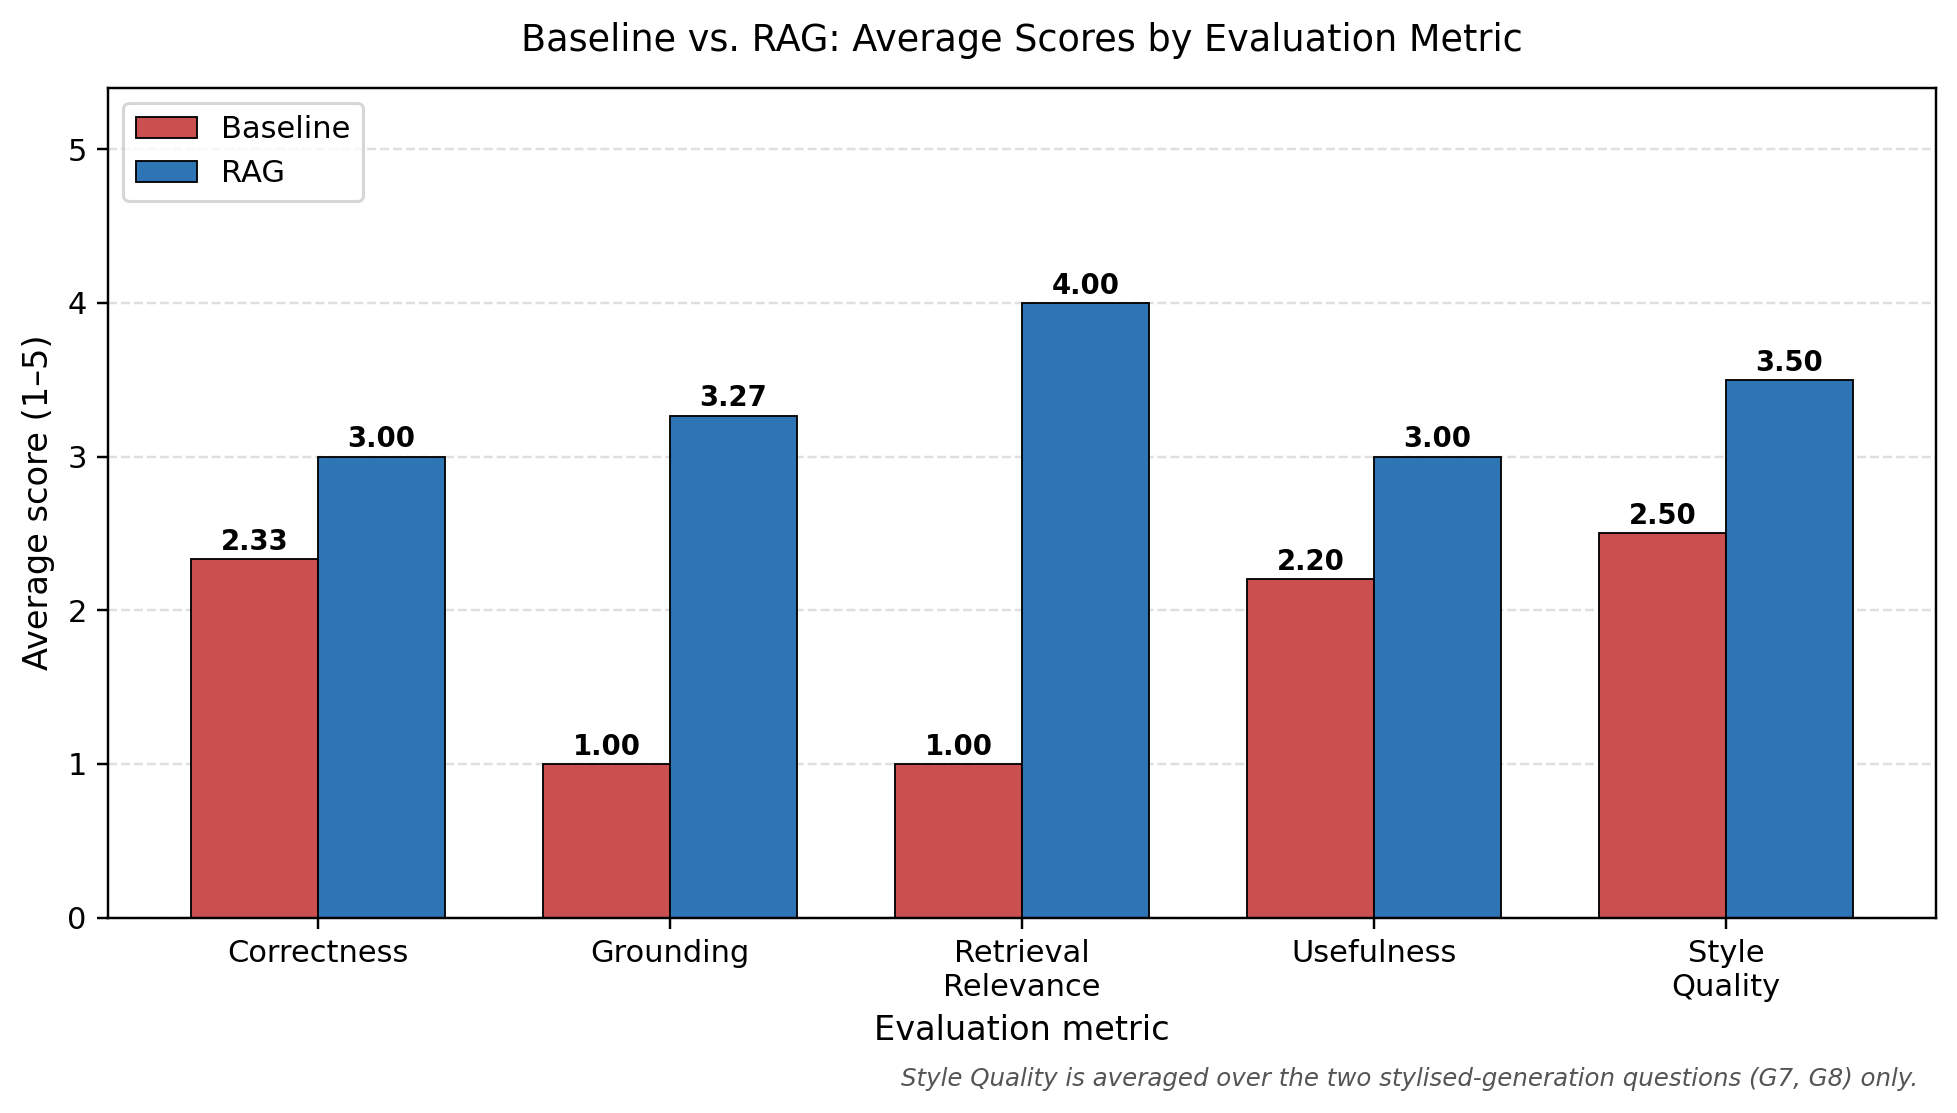
\includegraphics[width=\linewidth]{../report/figure1.png}
\caption{Average evaluation scores by metric for the Baseline and RAG systems. RAG outperforms the Baseline on every metric, with the largest gains on Retrieval Relevance (+3.00) and Grounding (+2.27).}
\label{fig:results-bar}
\end{figure}

\textbf{What we found:}

\begin{itemize}
    \item \textbf{RAG clearly improves grounding.} The baseline does not do any retrieval, so its grounding score is always 1. RAG answers often mention specific scenes, characters, and events from the retrieved passages, which is much better.
    \item \textbf{Retrieval works well for specific questions.} When the question is about a specific event (like Q1, Q5, G4, G6), the retriever usually finds the right scene. For example, Q1 gets Act~2 Scene~2 as the top result with a score of 0.740, which is exactly the scene where Macbeth kills Duncan.
    \item \textbf{RAG helps correctness, but hallucination still happens.} Even with the right context, TinyLlama sometimes makes up wrong details. For example, in Q1, the RAG answer says Duncan is ``the son of King Duncan and Queen Margaret,'' which is completely wrong.
    \item \textbf{Usefulness gets a bit better.} RAG answers are usually more specific and structured, but both systems can still be too long or repeat themselves.
\end{itemize}

\subsection{Qualitative Examples}

\textbf{Example 1: Successful retrieval and grounding (Q5).}

\textit{Question:} ``Why is Juliet conflicted after Romeo kills Tybalt?''

\textit{RAG retrieval:} The top result is Romeo and Juliet, Act~3 Scene~2 (score 0.669), which is exactly the scene where Juliet hears about Tybalt's death. The third result is Act~3 Scene~1, where the fight happens.

\textit{RAG answer:} ``Juliet is conflicted because she loves Romeo and is torn between her loyalty to her family and her feelings for him.'' This is correct for the main point. But the answer also says ``Juliet's conflicted emotions lead to her decision to leave Romeo and return to her family,'' which does not actually happen in the play.

\textit{Baseline answer:} The baseline gives a roughly correct but very general answer without any reference to the actual text.

\textit{Analysis:} RAG finds the right scene and gives a more specific answer, but the model still sometimes adds details that are not in the context.

\medskip

\textbf{Example 2: Evidence retrieval success (G4).}

\textit{Question:} ``What do the witches predict for Macbeth and Banquo?''

\textit{RAG retrieval:} The top result is Macbeth Act~1 Scene~3 (score 0.697), which is exactly where the witches tell their prophecies. This shows that for questions about specific events, the retrieval is quite accurate.

\medskip

\textbf{Example 3: Stylised generation (G7).}

\textit{Question:} ``Generate a short Shakespearean-style speech from Lady Macbeth urging Macbeth to seize the crown.''

\textit{RAG answer:} The system correctly adds the creative content label at the top. But the generated text is about 300 words, which is way over the 150-word limit. Also, it reads more like a modern letter than real Shakespearean English. This shows that it is very hard for a small model to control both the style and the length at the same time.

\subsection{Failure Analysis}

We found five main types of failures in our evaluation.

\textbf{Failure 1: Making up wrong plot details.}
In Q1, the RAG system says Duncan is ``the son of King Duncan and Queen Margaret,'' which is completely made up. In G6, it says Romeo and Juliet die of ``starvation,'' which is totally wrong (Romeo actually takes poison, and Juliet stabs herself). Even though the system retrieved the right scene (Act~5 Scene~1, score 0.631), the model did not use the information correctly.

\textit{Why this happens:} TinyLlama is a small model (only 1.1B parameters), so when the prompt is long, it has trouble following it properly and sometimes falls back to making things up.

\textbf{Failure 2: Mixing up different plays.}
For G5 (about the play-within-a-play), the baseline talks about \textit{Twelfth Night} instead of \textit{Hamlet}. The RAG system does find the right scene (Hamlet Act~3 Scene~2), but the answer it generates is messy and hard to follow.

\textit{Why this happens:} Without retrieval, the baseline model gets confused between different plays. With retrieval, we give it the right context, but the model's generation ability is still limited.

\textbf{Failure 3: Leaking the system prompt.}
For G9 (``Who is Mingzhao Zhu?''), the retrieval scores are all very low (top score is only 0.162), because there is nothing about this person in the plays. But instead of saying ``I don't know,'' the RAG model just copies the system prompt into the output. The baseline is even worse---it makes up a fake answer saying Mingzhao Zhu is ``a famous Chinese actor.''

\textit{Why this happens:} TinyLlama is not good at handling edge cases. When the context is not useful, it does not know what to do and just outputs whatever text it can find in the prompt.

\textbf{Failure 4: Stylised output is too long.}
For both G7 and G8, the stylised outputs are much longer than the 150-word limit. G7 is about 300 words, and G8 is even longer. Also, the writing style does not really sound like Shakespeare---it is more like modern English with a few old-fashioned words mixed in.

\textit{Why this happens:} Controlling the length and style of output is very hard for small models. The model sees the instruction about 150 words, but it cannot actually stop itself at that point.

\textbf{Failure 5: Retrieving passages from the wrong play.}
For Q6 (``How does the family feud shape the tragedy?''), the second-ranked result is from \textit{Macbeth} Act~1 Scene~1 (the witches scene), which has nothing to do with Romeo and Juliet. The similarity score for this result is only 0.414, which is quite low, but our retriever does not have a way to filter by play.

\textit{How to fix:} We could add a filter to only retrieve from the relevant play, or use some metadata-aware retrieval method.

% ============================================================
\section{Responsible Use of Generative AI}
\label{sec:genai}

We used Windsurf Cascade (which is powered by Claude) as a coding assistant during this project. Here is a summary of how we used it:

\textbf{What we used it for:}
\begin{itemize}
    \item Writing code: data loader, chunking, retrieval, RAG pipeline, evaluation script.
    \item Debugging: fixing environment problems like h5py DLL errors and TensorFlow import issues.
    \item Documentation: writing README files and drafting parts of this report.
    \item Discussing design choices: like which chunking strategy to use, which model to pick, and how to set up evaluation.
\end{itemize}

\textbf{How we checked the results:}
\begin{itemize}
    \item We ran all the generated code and checked the outputs to make sure they were correct.
    \item We read through the evaluation results to verify the system was working as expected.
    \item We reviewed the report content to make sure it matched what we actually implemented.
\end{itemize}

\textbf{What we changed or rejected:}
\begin{itemize}
    \item The AI suggested using FAISS for retrieval, but we decided cosine similarity with NumPy was enough for our small dataset, so we did not use FAISS.
    \item Some of the generated documentation was too wordy, so we edited it to be clearer.
\end{itemize}

The detailed GenAI usage log is in Appendix~\ref{app:genai-log}.

% ============================================================
\section{Conclusion}
\label{sec:conclusion}

In this project, we built a Shakespeare-aware RAG system using TinyLlama-1.1B-Chat for generation and MiniLM-L6-v2 for retrieval. The system can handle all four required interaction types, and we tested it with 15 questions across five categories.

\textbf{What went well:}
\begin{itemize}
    \item The retrieval part works quite well. For most questions, the top-1 result has a score above 0.6 and is the correct scene.
    \item RAG is clearly better than the prompt-only baseline, especially for grounding and retrieval relevance.
    \item The system can detect when the user wants stylised generation and adds the correct label to the output.
    \item The embedding cache makes the system start much faster after the first run.
\end{itemize}

\textbf{What did not go well:}
\begin{itemize}
    \item TinyLlama is too small (only 1.1B parameters) to follow instructions reliably. This causes hallucination, prompt leakage, and failure to control output length.
    \item The stylised generation does not really sound like Shakespeare.
    \item Sometimes the retriever returns passages from the wrong play.
    \item The system cannot handle out-of-domain questions well---it does not know how to say ``I don't know.''
\end{itemize}

\textbf{What we would do if we had more time:}
\begin{itemize}
    \item \textbf{Use a bigger model}: A 3B--7B model like Phi-2 or Mistral-7B (quantised) would generate much better answers and follow instructions more reliably.
    \item \textbf{Filter by play}: Add a filter so the retriever only searches in the relevant play when we can tell which play the question is about.
    \item \textbf{Re-ranking}: Use a cross-encoder to re-rank the retrieved results so the most relevant one is always on top.
    \item \textbf{Fine-tuning with LoRA}: Do some lightweight fine-tuning on Shakespeare QA data to make the model better at this specific task.
\end{itemize}

Overall, this project shows that RAG can really help a small model do better on domain-specific tasks. But it also shows that when the model is too small, there are clear limits to what you can achieve, no matter how good the retrieval is.

% ============================================================
% References
% ============================================================
\begin{thebibliography}{9}

\bibitem{tinyllama}
Z.~Zhang \textit{et al.}, ``TinyLlama: An Open-Source Small Language Model,'' \textit{arXiv preprint arXiv:2401.02385}, 2024.

\bibitem{minilm}
W.~Wang, F.~Wei, L.~Dong, H.~Bao, N.~Yang, and M.~Zhou, ``MiniLM: Deep Self-Attention Distillation for Task-Agnostic Compression of Pre-Trained Transformers,'' in \textit{Proc. NeurIPS}, 2020.

\bibitem{rag}
P.~Lewis \textit{et al.}, ``Retrieval-Augmented Generation for Knowledge-Intensive NLP Tasks,'' in \textit{Proc. NeurIPS}, 2020.

\bibitem{sentence-bert}
N.~Reimers and I.~Gurevych, ``Sentence-BERT: Sentence Embeddings using Siamese BERT-Networks,'' in \textit{Proc. EMNLP}, 2019.

\bibitem{gutenberg}
Project Gutenberg, ``Complete Works of William Shakespeare,'' \url{https://www.gutenberg.org/}.

\bibitem{lora}
E.~J.~Hu \textit{et al.}, ``LoRA: Low-Rank Adaptation of Large Language Models,'' in \textit{Proc. ICLR}, 2022.

\bibitem{hallucination}
Z.~Ji \textit{et al.}, ``Survey of Hallucination in Natural Language Generation,'' \textit{ACM Computing Surveys}, vol.~55, no.~12, 2023.

\end{thebibliography}

% ============================================================
% Appendices
% ============================================================
\appendices

\section{Full Evaluation Table}
\label{app:evaluation}

Table~\ref{tab:full-eval-baseline} and Table~\ref{tab:full-eval-rag} show the full evaluation results for the baseline and RAG systems. The score columns need to be filled in manually using the 1--5 rubric from Section~\ref{sec:evaluation-design}.

\begin{table*}[h]
\centering
\caption{Full evaluation results --- Baseline system. Fill in scores (1--5) manually.}
\label{tab:full-eval-baseline}
\begin{tabularx}{\textwidth}{llp{1.5cm}p{1.2cm}p{1.2cm}p{1.2cm}p{1.2cm}X}
\toprule
ID & Type & Corr. & Grnd. & Ret. & Use. & Style & Comments \\
\midrule
Q1 & ctx\_qa & 2 & 1 & N/A & 2 & N/A & No retrieval; mentions ambition vaguely but invents 'Duncan refuses to bow' detail; omits witches \& Lady Macbeth. \\
Q2 & ctx\_qa & 2 & 1 & N/A & 2 & N/A & Generic moralising tone; doesn't mention Banquo's murder, banquet scene, or paranoia. \\
Q3 & ctx\_qa & 3 & 1 & N/A & 2 & N/A & Long but generic; gives plot context but never actually answers WHY Hamlet delays. \\
Q4 & ctx\_qa & 3 & 1 & N/A & 3 & N/A & Treats Ophelia as generic tragic-love symbol; misses Polonius/Laertes/court politics aspects. \\
Q5 & ctx\_qa & 3 & 1 & N/A & 3 & N/A & Captures love/family tension at surface level; no textual evidence; misses kinsman aspect of Tybalt. \\
Q6 & ctx\_qa & 3 & 1 & N/A & 3 & N/A & Reasonable thematic answer about feud driving plot, but no specific evidence cited. \\
G1 & concept & 3 & 1 & N/A & 3 & N/A & Solid character summary of Lady Macbeth's role driving Macbeth's downfall, but no specific evidence. \\
G2 & concept & 2 & 1 & N/A & 2 & N/A & Major factual error: calls Claudius 'father of Gertrude'; he is her husband and Hamlet's uncle. \\
G3 & concept & 2 & 1 & N/A & 2 & N/A & Hallucinates Mercutio's death ('falls into a pit created by the Montagues') instead of being killed by Tybalt. \\
G4 & evidence & 2 & 1 & N/A & 2 & N/A & Incomplete and partly wrong: misses Thane of Cawdor + king prophecies; vague 'Banquo will have a son'. \\
G5 & evidence & 1 & 1 & N/A & 1 & N/A & Severe hallucination --- describes Twelfth Night plot (Viola/Olivia/Cesario) instead of Hamlet's Mousetrap. \\
G6 & ctx\_qa & 2 & 1 & N/A & 2 & N/A & Says Romeo 'kills himself' and Juliet 'dies of broken heart' --- partially right but missing poison/dagger and miscommunication. \\
G7 & stylised & 3 & 1 & N/A & 3 & 3 & Dialogue format with dramatic tone; reasonable Shakespearean register but no source grounding and no creative-output disclaimer. \\
G8 & stylised & 3 & 1 & N/A & 2 & 2 & Mostly modern English ('I sit here, surrounded by my family'); lacks Early Modern register and Hamlet's contemplative voice. \\
G9 & robust & 1 & 1 & N/A & 1 & N/A & Out-of-domain question, system cannot handle queries unrelated to Shakespeare \\
\bottomrule
\end{tabularx}
\end{table*}

\begin{table*}[h]
\centering
\caption{Full evaluation results --- RAG system. Fill in scores (1--5) manually.}
\label{tab:full-eval-rag}
\begin{tabularx}{\textwidth}{llp{1.5cm}p{1.2cm}p{1.2cm}p{1.2cm}p{1.2cm}X}
\toprule
ID & Type & Corr. & Grnd. & Ret. & Use. & Style & Comments \\
\midrule
Q1 & ctx\_qa & 3 & 4 & 4 & 3 & N/A & [Act 2.2 (0.74)] Retrieves correct Act 2.2 murder scene; partially uses evidence but fabricates 'son of King Duncan and Queen Margaret'. \\
Q2 & ctx\_qa & 3 & 3 & 4 & 3 & N/A & [Act 3.6 (0.62)] Retrieves Act 3.6 tyranny scene correctly, but answer wrongly claims Macbeth 'becomes compassionate and seeks forgiveness'. \\
Q3 & ctx\_qa & 3 & 3 & 3 & 3 & N/A & [Act 3.1 (0.59)] Retrieves Act 3.1 'To be or not to be'; mentions hesitation but invents claim that 'Polonius confirms Claudius is true king'. \\
Q4 & ctx\_qa & 3 & 4 & 4 & 3 & N/A & [Act 2.1 (0.62)] Retrieves Polonius/Reynaldo scene; mentions father's death, Laertes, suicide; describes plot impact reasonably. \\
Q5 & ctx\_qa & 4 & 4 & 5 & 4 & N/A & [Act 3.2 (0.67)] Retrieves the exact Act 3.2 Capulet's orchard scene; explicitly identifies family-loyalty conflict. \\
Q6 & ctx\_qa & 4 & 4 & 5 & 4 & N/A & [Prologue (0.56)] Retrieves the Prologue (perfect grounding choice); covers feud-deaths causal link explicitly. \\
G1 & concept & 3 & 3 & 4 & 3 & N/A & [Act 3.2 (0.61)] Retrieves Act 3.2 palace scene; mentions her letter and Cawdor reference, but mistakenly puts Cawdor title on her. \\
G2 & concept & 3 & 3 & 4 & 3 & N/A & [Act 3.3 (0.59)] Retrieves Act 3.3 prayer scene; correctly states he murdered Hamlet's father, but wrongly calls him 'father of Hamlet'. \\
G3 & concept & 4 & 4 & 5 & 4 & N/A & [Act 3.1 (0.56)] Retrieves Act 3.1 correctly; states Tybalt kills Mercutio leading to Romeo's revenge --- accurate and grounded. \\
G4 & evidence & 4 & 4 & 5 & 4 & N/A & [Act 1.3 (0.70)] Retrieves Act 1.3 heath scene; correctly identifies Banquo as 'root and father of many kings'. \\
G5 & evidence & 3 & 3 & 4 & 2 & N/A & [Act 3.2 (0.46)] Retrieves correct Act 3.2 scene but answer is incoherent --- quotes random fragments without explaining the trap on Claudius. \\
G6 & ctx\_qa & 1 & 2 & 5 & 1 & N/A & [Act 5.1 (0.63)] Retrieval is perfect (Act 5.1), but generation hallucinates that both die of starvation --- clear failure of grounding despite good retrieval. \\
G7 & stylised & 3 & 4 & 4 & 4 & 4 & [is\textbackslash\{\}\_stylised=True] Includes explicit creative-output disclaimer; opens with a real Macbeth quotation; clearly distinguished from factual answer. \\
G8 & stylised & 3 & 3 & 3 & 3 & 3 & [is\textbackslash\{\}\_stylised=True] Includes creative-output disclaimer and references Act 2.2; rambles into meta-description rather than producing a tight stylised speech. \\
G9 & robust & 1 & 1 & 1 & 1 & N/A & [score 0.16 (off-topic)] Out-of-domain question, system cannot handle queries unrelated to Shakespeare \\
\bottomrule
\end{tabularx}
\end{table*}

\section{Representative Prompts}
\label{app:prompts}

\subsection{RAG System Prompt}

\begin{lstlisting}[language={}]
You are a Shakespeare-aware assistant.

Use the retrieved context to answer the
user's question.
Your answer must be beginner-friendly.
If the retrieved context is insufficient,
say so clearly.
Do not invent unsupported details.
If asked to produce a Shakespearean-style
response, keep it under 150 words and make
clear that it is creative output, not
textual evidence.
\end{lstlisting}

\subsection{Baseline Prompt Template}

\begin{lstlisting}[language={}]
You are a helpful assistant that answers
questions about Shakespeare's plays.
Answer in a beginner-friendly way.
If you are unsure, say so.

Question: <user query>

Answer:
\end{lstlisting}

\subsection{Stylised Generation Prompt Template}

\begin{lstlisting}[language={}]
You are a creative writing assistant who
writes in Shakespearean style.
Based on the context below, write a SHORT
response (no more than 150 words) in the
style of Shakespeare. Use Early Modern
English vocabulary and poetic rhythm.
IMPORTANT: This is CREATIVE output, NOT
factual evidence. Make this clear in your
response.

Context:
<retrieved passages>

Request: <user query>

Shakespearean-style response (<=150 words):
\end{lstlisting}

\section{Additional Output Examples}
\label{app:outputs}

\subsection{Successful RAG Example: Q5}

\textbf{Question:} ``Why is Juliet conflicted after Romeo kills Tybalt?''

\textbf{Top retrieved passage:} Romeo and Juliet, Act 3, Scene 2, score = 0.669. Summary: ``Juliet learns Romeo killed Tybalt and is torn between love and family loyalty.''

\textbf{RAG response:} ``Juliet is conflicted after Romeo kills Tybalt because she loves Romeo and is torn between her loyalty to her family and her feelings for him. Romeo's actions towards Tybalt, who is a family friend, cause Juliet to feel anger, disgust, and sadness.''

\subsection{Failure Example: G9 (Out-of-Domain)}

\textbf{Question:} ``Who is Mingzhao Zhu?''

\textbf{Top retrieved passage:} Macbeth Act 5 Scene 9, score = 0.162 (very low, indicating no relevant content).

\textbf{RAG response:} The model outputs the entire system prompt verbatim instead of indicating that the question is outside its scope.

\textbf{Baseline response:} Fabricates: ``Mingzhao Zhu is a famous Chinese actor who has appeared in several Shakespearean plays.''

\subsection{Failure Example: G6 (Hallucinated Plot)}

\textbf{Question:} ``How do Romeo and Juliet die?''

\textbf{RAG response:} ``Romeo and Juliet die from the same cause: starvation.'' This is entirely incorrect. The correct answer (Romeo takes poison; Juliet stabs herself) was present in the retrieved context (Act 5 Scene 1) but the model failed to extract and use it.

\section{GenAI Usage Log}
\label{app:genai-log}

\begin{table*}[h]
\centering
\caption{GenAI usage log.}
\label{tab:genai-log}
\begin{tabularx}{\textwidth}{p{2.2cm} p{3.0cm} p{3.0cm} X}
\toprule
Tool & Prompt or Task & Useful Output & Verification / Modification \\
\midrule
Windsurf Cascade & Implement data loader for Shakespeare JSON files & Generated \texttt{data\_loader.py} with scene and utterance extraction & Tested with all 3 plays; verified record counts \\
\midrule
Windsurf Cascade & Implement scene-level chunking with summary enrichment & Generated \texttt{chunking.py} with long-scene splitting & Verified chunk counts and content manually \\
\midrule
Windsurf Cascade & Implement embedding caching in retrieval.py & Added disk-based caching with content hash & Tested cache hit/miss; verified hash invalidation \\
\midrule
Windsurf Cascade & Implement shared model loader (model.py) & Singleton pattern for TinyLlama loading & Verified model loads once across baseline and RAG \\
\midrule
Windsurf Cascade & Implement baseline system & Generated \texttt{baseline.py} with prompt-only generation & Tested with sample questions \\
\midrule
Windsurf Cascade & Implement RAG chatbot with stylised generation & Generated \texttt{rag\_chatbot.py} with auto-detection & Tested all 4 interaction types manually \\
\midrule
Windsurf Cascade & Implement evaluation script & Generated \texttt{evaluate.py} with CSV output & Ran full evaluation; verified 30-row CSV output \\
\midrule
Windsurf Cascade & Debug h5py DLL import error & Suggested fake module injection in config.py & Verified system runs without TensorFlow \\
\midrule
Windsurf Cascade & Write README files & Generated English and Chinese READMEs & Reviewed and corrected project structure details \\
\midrule
Windsurf Cascade & Draft technical report & Generated LaTeX report structure and content & Reviewed all claims against actual outputs; corrected evaluation scores and analysis \\
\bottomrule
\end{tabularx}
\end{table*}

\end{document}
